\documentclass[12pt]{article}

\usepackage{amsmath}
\usepackage{amssymb}
\usepackage{framed}
\usepackage{graphicx}
%opening

\begin{document}
\tableofcontents
\newpage
\section{Binomial Logistic Regression}

\subsection{Model Diagnostics}

\begin{itemize}
\item In order to understand how much variation in the dependent variable can be explained by the model (the equivalent of $R^2$ in multiple regression), you sho$R^2$uld consult Model Summary statistics.

\item The SPSS output table below contains the \textit{Cox \& Snell R Square} and \textit{Nagelkerke R Square }values, which are both methods of calculating the explained variation. These values are sometimes referred to as pseudo $R^2$ values (and will have lower values than in multiple regression).
\item  However, they are interpreted in the same manner, but with more caution. Therefore, the explained variation in the dependent variable based on our model ranges from 24.0\% to 33.0\%, depending on whether you reference the Cox \& Snell $R^2$ or Nagelkerke $R^2$ methods, respectively. 

\item Nagelkerke $R^2$ is a modification of Cox \& Snell $R^2$, the latter of which cannot achieve a value of 1. For this reason, it is preferable to report the Nagelkerke $R^2$ value.
\end{itemize}
\begin{figure}[h!]
\centering
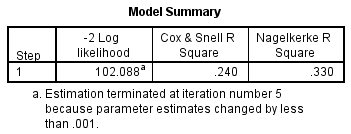
\includegraphics[width=0.9\linewidth]{BLogReg-Rsq}
\caption{SPSS output}
\label{fig:BLogReg-Rsq}
\end{figure}

\end{document}
